% Options for packages loaded elsewhere
\PassOptionsToPackage{unicode}{hyperref}
\PassOptionsToPackage{hyphens}{url}
\PassOptionsToPackage{dvipsnames,svgnames,x11names}{xcolor}
%
\documentclass[
  12pt,
  letterpaper,
  DIV=11,
  numbers=noendperiod]{scrartcl}

\usepackage{amsmath,amssymb}
\usepackage{iftex}
\ifPDFTeX
  \usepackage[T1]{fontenc}
  \usepackage[utf8]{inputenc}
  \usepackage{textcomp} % provide euro and other symbols
\else % if luatex or xetex
  \usepackage{unicode-math}
  \defaultfontfeatures{Scale=MatchLowercase}
  \defaultfontfeatures[\rmfamily]{Ligatures=TeX,Scale=1}
\fi
\usepackage{lmodern}
\ifPDFTeX\else  
    % xetex/luatex font selection
    \setmainfont[]{Times New Roman}
\fi
% Use upquote if available, for straight quotes in verbatim environments
\IfFileExists{upquote.sty}{\usepackage{upquote}}{}
\IfFileExists{microtype.sty}{% use microtype if available
  \usepackage[]{microtype}
  \UseMicrotypeSet[protrusion]{basicmath} % disable protrusion for tt fonts
}{}
\makeatletter
\@ifundefined{KOMAClassName}{% if non-KOMA class
  \IfFileExists{parskip.sty}{%
    \usepackage{parskip}
  }{% else
    \setlength{\parindent}{0pt}
    \setlength{\parskip}{6pt plus 2pt minus 1pt}}
}{% if KOMA class
  \KOMAoptions{parskip=half}}
\makeatother
\usepackage{xcolor}
\setlength{\emergencystretch}{3em} % prevent overfull lines
\setcounter{secnumdepth}{5}
% Make \paragraph and \subparagraph free-standing
\makeatletter
\ifx\paragraph\undefined\else
  \let\oldparagraph\paragraph
  \renewcommand{\paragraph}{
    \@ifstar
      \xxxParagraphStar
      \xxxParagraphNoStar
  }
  \newcommand{\xxxParagraphStar}[1]{\oldparagraph*{#1}\mbox{}}
  \newcommand{\xxxParagraphNoStar}[1]{\oldparagraph{#1}\mbox{}}
\fi
\ifx\subparagraph\undefined\else
  \let\oldsubparagraph\subparagraph
  \renewcommand{\subparagraph}{
    \@ifstar
      \xxxSubParagraphStar
      \xxxSubParagraphNoStar
  }
  \newcommand{\xxxSubParagraphStar}[1]{\oldsubparagraph*{#1}\mbox{}}
  \newcommand{\xxxSubParagraphNoStar}[1]{\oldsubparagraph{#1}\mbox{}}
\fi
\makeatother

\usepackage{color}
\usepackage{fancyvrb}
\newcommand{\VerbBar}{|}
\newcommand{\VERB}{\Verb[commandchars=\\\{\}]}
\DefineVerbatimEnvironment{Highlighting}{Verbatim}{commandchars=\\\{\}}
% Add ',fontsize=\small' for more characters per line
\usepackage{framed}
\definecolor{shadecolor}{RGB}{241,243,245}
\newenvironment{Shaded}{\begin{snugshade}}{\end{snugshade}}
\newcommand{\AlertTok}[1]{\textcolor[rgb]{0.68,0.00,0.00}{#1}}
\newcommand{\AnnotationTok}[1]{\textcolor[rgb]{0.37,0.37,0.37}{#1}}
\newcommand{\AttributeTok}[1]{\textcolor[rgb]{0.40,0.45,0.13}{#1}}
\newcommand{\BaseNTok}[1]{\textcolor[rgb]{0.68,0.00,0.00}{#1}}
\newcommand{\BuiltInTok}[1]{\textcolor[rgb]{0.00,0.23,0.31}{#1}}
\newcommand{\CharTok}[1]{\textcolor[rgb]{0.13,0.47,0.30}{#1}}
\newcommand{\CommentTok}[1]{\textcolor[rgb]{0.37,0.37,0.37}{#1}}
\newcommand{\CommentVarTok}[1]{\textcolor[rgb]{0.37,0.37,0.37}{\textit{#1}}}
\newcommand{\ConstantTok}[1]{\textcolor[rgb]{0.56,0.35,0.01}{#1}}
\newcommand{\ControlFlowTok}[1]{\textcolor[rgb]{0.00,0.23,0.31}{\textbf{#1}}}
\newcommand{\DataTypeTok}[1]{\textcolor[rgb]{0.68,0.00,0.00}{#1}}
\newcommand{\DecValTok}[1]{\textcolor[rgb]{0.68,0.00,0.00}{#1}}
\newcommand{\DocumentationTok}[1]{\textcolor[rgb]{0.37,0.37,0.37}{\textit{#1}}}
\newcommand{\ErrorTok}[1]{\textcolor[rgb]{0.68,0.00,0.00}{#1}}
\newcommand{\ExtensionTok}[1]{\textcolor[rgb]{0.00,0.23,0.31}{#1}}
\newcommand{\FloatTok}[1]{\textcolor[rgb]{0.68,0.00,0.00}{#1}}
\newcommand{\FunctionTok}[1]{\textcolor[rgb]{0.28,0.35,0.67}{#1}}
\newcommand{\ImportTok}[1]{\textcolor[rgb]{0.00,0.46,0.62}{#1}}
\newcommand{\InformationTok}[1]{\textcolor[rgb]{0.37,0.37,0.37}{#1}}
\newcommand{\KeywordTok}[1]{\textcolor[rgb]{0.00,0.23,0.31}{\textbf{#1}}}
\newcommand{\NormalTok}[1]{\textcolor[rgb]{0.00,0.23,0.31}{#1}}
\newcommand{\OperatorTok}[1]{\textcolor[rgb]{0.37,0.37,0.37}{#1}}
\newcommand{\OtherTok}[1]{\textcolor[rgb]{0.00,0.23,0.31}{#1}}
\newcommand{\PreprocessorTok}[1]{\textcolor[rgb]{0.68,0.00,0.00}{#1}}
\newcommand{\RegionMarkerTok}[1]{\textcolor[rgb]{0.00,0.23,0.31}{#1}}
\newcommand{\SpecialCharTok}[1]{\textcolor[rgb]{0.37,0.37,0.37}{#1}}
\newcommand{\SpecialStringTok}[1]{\textcolor[rgb]{0.13,0.47,0.30}{#1}}
\newcommand{\StringTok}[1]{\textcolor[rgb]{0.13,0.47,0.30}{#1}}
\newcommand{\VariableTok}[1]{\textcolor[rgb]{0.07,0.07,0.07}{#1}}
\newcommand{\VerbatimStringTok}[1]{\textcolor[rgb]{0.13,0.47,0.30}{#1}}
\newcommand{\WarningTok}[1]{\textcolor[rgb]{0.37,0.37,0.37}{\textit{#1}}}

\providecommand{\tightlist}{%
  \setlength{\itemsep}{0pt}\setlength{\parskip}{0pt}}\usepackage{longtable,booktabs,array}
\usepackage{calc} % for calculating minipage widths
% Correct order of tables after \paragraph or \subparagraph
\usepackage{etoolbox}
\makeatletter
\patchcmd\longtable{\par}{\if@noskipsec\mbox{}\fi\par}{}{}
\makeatother
% Allow footnotes in longtable head/foot
\IfFileExists{footnotehyper.sty}{\usepackage{footnotehyper}}{\usepackage{footnote}}
\makesavenoteenv{longtable}
\usepackage{graphicx}
\makeatletter
\newsavebox\pandoc@box
\newcommand*\pandocbounded[1]{% scales image to fit in text height/width
  \sbox\pandoc@box{#1}%
  \Gscale@div\@tempa{\textheight}{\dimexpr\ht\pandoc@box+\dp\pandoc@box\relax}%
  \Gscale@div\@tempb{\linewidth}{\wd\pandoc@box}%
  \ifdim\@tempb\p@<\@tempa\p@\let\@tempa\@tempb\fi% select the smaller of both
  \ifdim\@tempa\p@<\p@\scalebox{\@tempa}{\usebox\pandoc@box}%
  \else\usebox{\pandoc@box}%
  \fi%
}
% Set default figure placement to htbp
\def\fps@figure{htbp}
\makeatother
% definitions for citeproc citations
\NewDocumentCommand\citeproctext{}{}
\NewDocumentCommand\citeproc{mm}{%
  \begingroup\def\citeproctext{#2}\cite{#1}\endgroup}
\makeatletter
 % allow citations to break across lines
 \let\@cite@ofmt\@firstofone
 % avoid brackets around text for \cite:
 \def\@biblabel#1{}
 \def\@cite#1#2{{#1\if@tempswa , #2\fi}}
\makeatother
\newlength{\cslhangindent}
\setlength{\cslhangindent}{1.5em}
\newlength{\csllabelwidth}
\setlength{\csllabelwidth}{3em}
\newenvironment{CSLReferences}[2] % #1 hanging-indent, #2 entry-spacing
 {\begin{list}{}{%
  \setlength{\itemindent}{0pt}
  \setlength{\leftmargin}{0pt}
  \setlength{\parsep}{0pt}
  % turn on hanging indent if param 1 is 1
  \ifodd #1
   \setlength{\leftmargin}{\cslhangindent}
   \setlength{\itemindent}{-1\cslhangindent}
  \fi
  % set entry spacing
  \setlength{\itemsep}{#2\baselineskip}}}
 {\end{list}}
\usepackage{calc}
\newcommand{\CSLBlock}[1]{\hfill\break\parbox[t]{\linewidth}{\strut\ignorespaces#1\strut}}
\newcommand{\CSLLeftMargin}[1]{\parbox[t]{\csllabelwidth}{\strut#1\strut}}
\newcommand{\CSLRightInline}[1]{\parbox[t]{\linewidth - \csllabelwidth}{\strut#1\strut}}
\newcommand{\CSLIndent}[1]{\hspace{\cslhangindent}#1}

\usepackage{tcolorbox}
\usepackage{amssymb}
\usepackage{yfonts}
\usepackage{bm}


\newtcolorbox{greybox}{
  colback=white,
  colframe=blue,
  coltext=black,
  boxsep=5pt,
  arc=4pt}
  
\newcommand{\sectionbreak}{\clearpage}

 
\newcommand{\ds}[4]{\sum_{{#1}=1}^{#3}\sum_{{#2}=1}^{#4}}
\newcommand{\us}[3]{\mathop{\sum\sum}_{1\leq{#2}<{#1}\leq{#3}}}

\newcommand{\ol}[1]{\overline{#1}}
\newcommand{\ul}[1]{\underline{#1}}

\newcommand{\amin}[1]{\mathop{\text{argmin}}_{#1}}
\newcommand{\amax}[1]{\mathop{\text{argmax}}_{#1}}

\newcommand{\ci}{\perp\!\!\!\perp}

\newcommand{\mc}[1]{\mathcal{#1}}
\newcommand{\mb}[1]{\mathbb{#1}}
\newcommand{\mf}[1]{\mathfrak{#1}}

\newcommand{\eps}{\epsilon}
\newcommand{\lbd}{\lambda}
\newcommand{\alp}{\alpha}
\newcommand{\df}{=:}
\newcommand{\am}[1]{\mathop{\text{argmin}}_{#1}}
\newcommand{\ls}[2]{\mathop{\sum\sum}_{#1}^{#2}}
\newcommand{\ijs}{\mathop{\sum\sum}_{1\leq i<j\leq n}}
\newcommand{\jis}{\mathop{\sum\sum}_{1\leq j<i\leq n}}
\newcommand{\sij}{\sum_{i=1}^n\sum_{j=1}^n}
	
\KOMAoption{captions}{tableheading}
\makeatletter
\@ifpackageloaded{caption}{}{\usepackage{caption}}
\AtBeginDocument{%
\ifdefined\contentsname
  \renewcommand*\contentsname{Table of contents}
\else
  \newcommand\contentsname{Table of contents}
\fi
\ifdefined\listfigurename
  \renewcommand*\listfigurename{List of Figures}
\else
  \newcommand\listfigurename{List of Figures}
\fi
\ifdefined\listtablename
  \renewcommand*\listtablename{List of Tables}
\else
  \newcommand\listtablename{List of Tables}
\fi
\ifdefined\figurename
  \renewcommand*\figurename{Figure}
\else
  \newcommand\figurename{Figure}
\fi
\ifdefined\tablename
  \renewcommand*\tablename{Table}
\else
  \newcommand\tablename{Table}
\fi
}
\@ifpackageloaded{float}{}{\usepackage{float}}
\floatstyle{ruled}
\@ifundefined{c@chapter}{\newfloat{codelisting}{h}{lop}}{\newfloat{codelisting}{h}{lop}[chapter]}
\floatname{codelisting}{Listing}
\newcommand*\listoflistings{\listof{codelisting}{List of Listings}}
\usepackage{amsthm}
\theoremstyle{plain}
\newtheorem{lemma}{Lemma}[section]
\theoremstyle{remark}
\AtBeginDocument{\renewcommand*{\proofname}{Proof}}
\newtheorem*{remark}{Remark}
\newtheorem*{solution}{Solution}
\newtheorem{refremark}{Remark}[section]
\newtheorem{refsolution}{Solution}[section]
\makeatother
\makeatletter
\makeatother
\makeatletter
\@ifpackageloaded{caption}{}{\usepackage{caption}}
\@ifpackageloaded{subcaption}{}{\usepackage{subcaption}}
\makeatother

\usepackage{bookmark}

\IfFileExists{xurl.sty}{\usepackage{xurl}}{} % add URL line breaks if available
\urlstyle{same} % disable monospaced font for URLs
\hypersetup{
  pdfauthor={Jan de Leeuw},
  colorlinks=true,
  linkcolor={blue},
  filecolor={Maroon},
  citecolor={Blue},
  urlcolor={Blue},
  pdfcreator={LaTeX via pandoc}}


\title{Smacof at 50: A Manual\\
Part 1: The Basics}
\author{Jan de Leeuw}
\date{December 8, 2024}

\begin{document}
\maketitle

\renewcommand*\contentsname{Table of contents}
{
\hypersetup{linkcolor=}
\setcounter{tocdepth}{3}
\tableofcontents
}

\textbf{Note:} This is a working manuscript which will be
expanded/updated frequently. All suggestions for improvement are
welcome. All Rmd, tex, html, pdf, R, and C files are in the public
domain. Attribution will be appreciated, but is not required. The files
can be found at \url{https://github.com/deleeuw} in the repositories
smacofCode, smacofManual, and smacofExamples.

\sectionbreak

\section{Loss Function}\label{loss-function}

In the pioneering papers Kruskal (\citeproc{ref-kruskal_64a}{1964a}) and
Kruskal (\citeproc{ref-kruskal_64b}{1964b}) the MDS problem was
formulated for the first time as minimization of an explicit \emph{loss
function} or \emph{badness-of-fit function}, which measures the quality
of the approximation of the dissimilarities by the distances. To be
historically accurate, we should mention that the non-metric MDS
technique proposed by Shepard (\citeproc{ref-shepard_62a}{1962a}) and
Shepard (\citeproc{ref-shepard_62b}{1962b}) can be reformulated as
minimization of an explicit loss function (see, for example, De Leeuw
(\citeproc{ref-deleeuw_E_17e}{2017})). And the classical
Young-Householder-Torgerson MDS technique (Torgerson
(\citeproc{ref-torgerson_52}{1952})) for metric MDS can be reformulated
as minimizing an explicit least squares loss function (De Leeuw and
Heiser (\citeproc{ref-deleeuw_heiser_C_82}{1982})) as well. But neither
of these two predecessors was formulated originally as an explicit
minimization problem for a specific loss function

\subsection{Metric MDS}\label{metric-mds}

The loss function in least squares metric Euclidean MDS is called
\emph{raw stress} and is defined as \begin{equation}
\sigma_R(X):=\frac12\mathop{\sum\sum}_{1\leq j<i\leq n}w_{ij}(\delta_{ij}-d_{ij}(X))^2.
(\#eq:stressdef)
\end{equation} The subscript R in \(\sigma_R\) stands for ``raw'',
because we will discuss other least squares loss functions for which we
will also use the symbol \(\sigma\), but with other subscripts.

In definition @ref(eq:stressdef) the \(w_{ij}\) are known non-negative
\emph{weights}, the \(\delta_{ij}\) are the known non-negative
\emph{dissimilarities} between objects \(o_i\) and \(o_j\), and the
\(d_{ij}(X)\) are the \emph{distances} between the corresponding points
\(x_i\) and \(x_j\). The summation is over all pairs \((i,j)\) with
\(w_{ij}>0\). From now on we use ``metric MDS'' to mean the minimization
of \(\sigma_R\).

The \(n\times p\) matrix \(X\), which has the coordinates \(x_i\) of the
\(n\) points as its rows, is called the \emph{configuration}, where
\(p\) is the \emph{dimension} of the Euclidean space in which we make
the map. The metric MDS problem (of dimension \(p\), for given \(W\) and
\(\Delta\)) is the minimization of @ref(eq:stressdef) over the
\(n\times p\) configurations \(X\).

The weights \(w_{ij}\) can be used to quantify information about the
precision or importance of the corresponding dissimilarities. Some of
the weights may be zero, which can be used to code \emph{missing data}.
If all weights are positive we have \emph{complete data}. If we have
complete data, and all weights are equal to one, we have
\emph{unweighted} metric MDS. The pioneering papers by Shepard, Kruskal,
and Guttman only consider the unweighted case. Weights were only
introduced in MDS in De Leeuw (\citeproc{ref-deleeuw_C_77}{1977}).

We assume throughout that the weights are \emph{irreducible} (De Leeuw
(\citeproc{ref-deleeuw_C_77}{1977})). This means there is no
partitioning of the index set \(I_n:=\{1,2,\cdots,n\}\) into subsets for
which all between-subset weights are zero. A reducible metric MDS
problems decomposes into a number of smaller independent metric MDS
problems, so the irreducibility assumption causes no real loss of
generality.

The fact that the summation in @ref(eq:stressdef) is over all \(j<i\)
indicates that the diagonal elements of \(\Delta\) are not used (they
are assumed to be zero) and the elements above the diagonal are not used
either (they are assumed to be equal to the corresponding elements below
the diagonal). The somewhat mysterious factor \(\frac12\) in definition
@ref(eq:stressdef) is there because it simplifies some of the formulas
in later sections of this paper.

\subsection{Non-linear MDS}\label{non-linear-mds}

Kruskal was not really interested in metric MDS and the ``raw'' loss
function @ref(eq:stressdef). His papers are really about non-metric MDS,
by which we mean least squares non-metric Euclidean MDS. Non-metric MDS
differs from metric MDS because we have incomplete information about the
dissimilarities. As we have seen, that if some dissimilarities are
missing metric MDS can handle this by using zero weights. In some
situations, however, we only know the rank order of the non-missing
dissimilarities. We do not know, or we refuse to use, their actual
numeric values. Or, to put it differently, even if we have numerical
dissimilarities we are looking for a \emph{transformation} of the
non-missing dissimilarities, where the transformation is chosen from a
set of admissible transformations (for instance from all linear or
monotone transformations). If the dissimilarities are non-numerical, for
example rank orders or partitionings, we choose from the set of
admissible \emph{quantifications}.

In non-metric MDS raw stress becomes \begin{equation}
\sigma_R(X,\Delta):=\frac12\sum w_{ij}(\delta_{ij}-d_{ij}(X))^2,
(\#eq:rawstressdef)
\end{equation} where \(\Delta\) varies over the quantified or
transformed dissimilarities. In MDS parlance they are also called
\emph{pseudo-distances} or \emph{disparities}. Loss function
@ref(eq:rawstressdef) must be minimized over both configurations and
disparities, with the condition that the disparities \(\Delta\) are an
admissible transformation or quantification of the data. In Kruskal's
non-metric MDS this means requiring monotonicity. In this paper we will
consider various other choices for the set of admissible
transformations. We will use the symbol \(\mathfrak{D}\) for the set of
admissible transformations

The most familiar examples of \(\mathfrak{D}\) (linear, polynomial,
splines, monotone) define convex cones with apex at the origin. This
means that if \(\Delta\in\mathfrak{D}\) then so is \(\lambda\Delta\) for
all \(\lambda\geq 0\). But consequently minimizing @ref(eq:rawstressdef)
over all \(\Delta\in\mathfrak{D}\) and over all configurations has the
trivial solution \(\Delta=0\) and \(X=0\), corresponding with the global
minimum \(\sigma(X,\Delta)=0\). We need additional constraints to rule
out this trivial solution, and in non-metric MDS this is done by
choosing a \emph{normalization} that keeps the solution away from zero.

Kruskal's original solution is to define \emph{normalized stress} as
\begin{equation}
\sigma(X,\Delta):=\frac{\sum w_{ij}(\delta_{ij}-d_{ij}(X))^2}{\sum w_{ij}d_{ij}^2(X)}.
(\#eq:nstressdef)
\end{equation} To be precise, in Kruskal's formulation there are no
weights, and he actually takes the square root of @ref(eq:nstressdef) to
define \emph{Kruskal's stress}. The non-metric Euclidean MDS problem now
is to minimize loss function @ref(eq:nstressdef) over all \(n\times p\)
configurations \(X\) and all admissible disparities \(\Delta\).

\subsection{Non-metric MDS}\label{non-metric-mds}

\subsection{Normalization}\label{normalization}

Equation @ref(eq:nstressdef) is only one way to normalize raw stress.
Some obvious alternatives are discussed in detail in Kruskal and Carroll
(\citeproc{ref-kruskal_carroll_69}{1969}) and De Leeuw
(\citeproc{ref-deleeuw_U_75a}{1975}). In the terminology of De Leeuw
(\citeproc{ref-deleeuw_U_75a}{1975}) there are \emph{explicit} and
\emph{implicit} normalizations.

In implicit normalization we minimize either \begin{equation}
\sigma(X,\hat D):=\frac{\sum  w_{ij}(\hat d_{ij} -d_{ij}(X))^2}{\sum   w_{ij}^{\ }\hat d_{ij}^2}
(\#eq:implicit1)
\end{equation} or \begin{equation}
\sigma(X,\hat D):=\frac{\sum   w_{ij}(\hat d_{ij}-d_{ij}(X))^2}{\sum   w_{ij}^{\ }d_{ij}^2(X) }
(\#eq:implicit2)
\end{equation} over \(X\) and \(\Delta\in\mathfrak{D}\).

As we have seen, Kruskal (\citeproc{ref-kruskal_64a}{1964a}) chooses
definition @ref(eq:implicit2) and calls the explicitly normalized loss
function \emph{normalized stress}. Note that we overload the symbol
\(\sigma\) to denote any one of the least squares loss functions. It
will always be clear from the text which \(\sigma\) we are talking
about.

In explicit normalization we minimize the raw stress
\(\sigma_R(X,\hat D)\) from @ref(eq:rawstressdef), but we add the
explicit constraint \begin{equation}
\sum   w_{ij}^{\ }d_{ij}^2(X)=1,
(\#eq:explicit1)
\end{equation} or the constraint \begin{equation}
\sum   w_{ij}^{\ }\hat d_{ij}^2=1.
(\#eq:explicit2)
\end{equation} Kruskal and Carroll
(\citeproc{ref-kruskal_carroll_69}{1969}) and De Leeuw
(\citeproc{ref-deleeuw_E_19d}{2019}) show that these four normalizations
all lead to essentially the same solution for \(X\) and \(\hat D\), up
to scale factors dictated by the choice of the particular normalization.
It is also possible to normalize both \(X\) and \(\hat D\), either
explicitly or implicitly, and again this will give the same solutions,
suitably normalized. These invariance results assume the admissible
transformations form a closed cone with apex at the origin, i.e.~if
\(\hat D\) is admissible and \(\lambda\geq 0\) then \(\lambda\hat D\) is
admissible as well. The matrices of Euclidean distances \(D(X)\) form a
similar closed cone as well. The non-metric MDS problem is to find an
element of the \(\hat D\) cone \(\mathcal{D}\) and an element of the
\(D(X)\) cone where the angle between the two is a small as possible.

In the R version of smacof (De Leeuw and Mair
(\citeproc{ref-deleeuw_mair_A_09c}{2009}), Mair, Groenen, and De Leeuw
(\citeproc{ref-mair_groenen_deleeuw_A_22}{2022})) we use explicit
normalization @ref(eq:explicit2). This is supported by the result, also
due to De Leeuw (\citeproc{ref-deleeuw_U_75a}{1975}), that projection on
the intersection of the cone of disparities and the sphere defined by
@ref(eq:explicit2) is equivalent to first projecting on the cone and
then normalizing the projection (see also Bauschke, Bui, and Wang
(\citeproc{ref-bauschke_bui_wang_18}{2018})).

In the version of non-metric MDS discussed in this manual we need more
flexibility. For algorithmic reasons that may become clear later on, we
will go with the original @ref(eq:nstressdef), i.e.~with the implicitly
normalized Kruskal's stress. For the final results the choice between
normalizations should not make a difference, but the iterative
computations will be different for the different choices.

\subsection{Some thoughts on ALS}\label{some-thoughts-on-als}

The formulation in equations @ref(eq:gmdsdef1) and @ref(eq:gmdsdef2)
neatly separates the metric MDS part @ref(eq:gmdsdef1) and the
transformation/quantification part @ref(eq:gmdsdef2). This second part
is also often called the \emph{optimal scaling} part.

Equations @ref(eq:gmdsdef1) and @ref(eq:gmdsdef2) corresponds with the
way most iterative non-linear and non-metric MDS techniques are
implemented. The algorithms use \emph{Alternating Least Squares} (ALS).
There have been quite a few ALS algorithms avant-la-lettre, but as far
as I know both the name and ALS as a general approach to algorithm
construction were first introduced in De Leeuw
(\citeproc{ref-deleeuw_R_68d}{1968}), and then widely disseminated in a
series of papers by De Leeuw, Young, and Takane in the 1970's (work
summarized in Young, De Leeuw, and Takane
(\citeproc{ref-young_deleeuw_takane_C_80}{1980}) and Young
(\citeproc{ref-young_81}{1981})).

In the ALS implementation of MDS two sub-algorithms are used in each
iteration: one to improve the fit of the distances to the current
disparities \(\Delta\) and one to improve the fit of the disparities to
the current distances. The two sub-algorithms define one major iteration
of the MDS technique. In formulas (using superscript \((k)\) for major
iteration number) we start with \((X^{(0)},\Delta^{(0)})\) and then
alternate the mimization problems \begin{subequations}
\begin{align}
X^{(k+1)}&\ni\{\sigma(X^{(k+1)},\Delta^{(k)})=\min_{X\in\mathfrak{X}}\sigma(X,\Delta^{(k)})\},\\
\Delta^{(k+1)}&\ni\{\sigma(X^{(k+1)},\Delta^{(k+1)})=\min_{\Delta\in\mathfrak{D}}\sigma(X^{(k+1)},\Delta)\},
\end{align}
\end{subequations} where \(\ni\) is short for ``such that''. In MDS it
is more realistic not to minimize loss in the sub-steps but merely to
decrease it. Minimization in one or both of the two subproblems may
itself require an infinite iterative method, which we have to truncate
anyway. Thus \begin{subequations}
\begin{align}
X^{(k+1)}\in\mathfrak{X}&\ni\{\sigma(X^{(k+1)},\Delta^{(k)})<\sigma(X^{(k)},\Delta^{(k)})\},\\
\Delta^{(k+1)}\in\mathfrak{D}&\ni\{\sigma(X^{(k+1)},\Delta^{(k+1)})<\sigma(X^{(k+1)},\Delta^{(k)})\}.
\end{align}
\end{subequations}

\subsubsection{The Single-Phase
approach}\label{the-single-phase-approach}

In Kruskal (\citeproc{ref-kruskal_64a}{1964a}) defines \begin{equation}
\sigma(X):=\min_{\hat D\in\mathfrak{D}}\ \sigma(\hat D,X)=\sigma(X,\hat D(X)),
(\#eq:project)
\end{equation} where \(\sigma(\hat D,X)\) is defined by
@ref(eq:implicit2). The minimum in @ref(eq:project) is over admissible
transformations. In definition @ref(eq:project) \begin{equation}
\hat D(X):=\mathop{\text{argmin}}_{\hat D\in\mathfrak{D}}\sigma(X, \hat D).
(\#eq:optscal)
\end{equation} Normalized stress defined by @ref(eq:project) is now a
function of \(X\) only. Under some conditions, which are true in
Kruskal's definition of non-metric MDS, there is a simple relation
between the partials of @ref(eq:implicit2) and those of
@ref(eq:project). \begin{equation}
\mathcal{D}\sigma(X)=\mathcal{D}_1\sigma(X,\hat D(X)),
(\#eq:partials)
\end{equation} where \(\mathcal{D}\sigma(X)\) are the derivatives of
\(\sigma\) from @ref(eq:project) and
\(\mathcal{D}_1\sigma(X,\hat D(X))\) are the partial derivatives of
\(\sigma\) from @ref(eq:implicit2) with respect to \(X\). Thus the
partials of \(\sigma\) from @ref(eq:project) can be computed by
evaluating the partials of \(\sigma\) from @ref(eq:implicit2) with
respect to \(X\) at \((X,\hat D(X))\). This has created much confusion
in the past. The non-metric MDS problem in Kruskal's original
formulation is now to minimize \(\sigma\) from @ref(eq:project), which
is a function of \(X\) alone.

Guttman (\citeproc{ref-guttman_68}{1968}) calls this the
\emph{single-phase approach}. A variation of Kruskal's single-phase
approach defines \begin{equation}
\sigma(X)=\sum w_{ij}(d_{ij}^\#(X)-d_{ij}(X))^2,
(\#eq:rankimage)
\end{equation} where the \(d_{ij}^\#(X)\) are \emph{Guttman's rank
images}, i.e.~the permutation of the \(d_{ij}(X)\) that makes them
monotone with the \(\delta_{ij}\) (Guttman
(\citeproc{ref-guttman_68}{1968})). Or, alternatively, define
\begin{equation}
\sigma(X):=\sum   w_{ij}(d_{ij}^\%(X)-d_{ij}(X))^2,
(\#eq:shepard)
\end{equation} where the \(\hat d_{ij}^\%(X)\) are \emph{Shepard's rank
images}, i.e.~the permutation of the \(\delta_{ij}\) that makes them
monotone with the \(d_{ij}(X)\) (Shepard
(\citeproc{ref-shepard_62a}{1962a}), Shepard
(\citeproc{ref-shepard_62b}{1962b}), De Leeuw
(\citeproc{ref-deleeuw_E_17e}{2017})).

Minimizing the Shepard or Guttman single-phase loss functions is
computationally more complicated than Kruskal's \emph{monotone
regression} approach, mostly because the rank-image transformations are
not differentiable, and there is no analog of @ref(eq:partials) and of
the equivalence of the different implicit and explicit normalizations.

\subsubsection{The Two-Phase Approach}\label{the-two-phase-approach}

The \emph{two-phase approach} or \emph{alternating least squares (ALS)}
approach alternates minimization of \(\sigma(\hat D,X)\) over \(X\) for
our current best estimate of \(\hat D\) with minimization of
\(\sigma(\hat D,X)\) over \(\Delta\in\mathfrak{D}\) for our current best
value of \(X\). Thus an update from iteration \(k\) to iteration \(k+1\)
looks like \begin{subequations}
\begin{align}
\hat D^{(k)}&=\mathop{\text{argmin}}_{\hat D\in\mathfrak{D}}\sigma(\hat D,X^{(k)}),(\#eq:step1)\\
X^{(k+1)}&=\mathop{\text{argmin}}_X\sigma(\hat D^{(k)},X).(\#eq:step2)
\end{align} 
\end{subequations} This ALS approach to MDS was in the air since the
early (unsuccessful) attempts around 1968 of Young and De Leeuw to
combine Torgerson's classic metric MDS method with Kruskal's monotone
regression transformation. All previous implementations of non-metric
smacof use the two-phase approach, and we will do the same in this
paper.

As formulated, however, there are some problems with the ALS algorithm.
Step @ref(eq:step1) is easy to carry out, using monotone regression.
Step @ref(eq:step2) means solving a metric scaling problem, which is an
iterative proces that requires an infinite number of iterations. Thus,
in the usual implementations, step @ref(eq:step1) is combined with one
of more iterations of a convergent iterative procedure for metric MDS,
such as smacof. If we take only one of these \emph{inner iterations} the
algorithm becomes indistinguishable from Kruskal's single-phase method.
This has also created much confusion in the past.

In the usual implementations of the ALS approach we solve the first
subproblem @ref(eq:step1) exactly, while we take only a single step
towards the solution for given \(\hat D\) in the second phase
@ref(eq:step2). If we have an infinite iterative procedure to compute
the optimal \(\hat D\in\mathfrak{D}\) for given \(X\), then a more
balanced approach would be to take several inner iterations in the first
phase and several inner iterations in the second phase. How many of
each, nobody knows. In our current implementation of smacof we take
several inner iteration steps in the first phase and a single inner
iteration step in the second phase.

\sectionbreak

\section{Smacof Notation and
Terminology}\label{smacof-notation-and-terminology}

We discuss some the MDS notation used in smacof, which was first
introduced in De Leeuw (\citeproc{ref-deleeuw_C_77}{1977}) and De Leeuw
and Heiser (\citeproc{ref-deleeuw_heiser_C_77}{1977}). More detailed De
Leeuw and Heiser (\citeproc{ref-deleeuw_heiser_C_80}{1980}), De Leeuw
(\citeproc{ref-deleeuw_A_88b}{1988}), Borg and Groenen
(\citeproc{ref-borg_groenen_05}{2005}), Groenen and Van de Velden
(\citeproc{ref-groenen_vandevelden_16}{2016})

This notation is useful for the second phase of the ALS algorithm, in
which solve the metric MDS problem of we minimizing unnormalized
\(\sigma(X,\hat D)\) over \(X\) for fixed \(\hat D\). We will discuss
the first ALS phase later in the paper.

Start with the unit vectors \(e_i\) of length \(n\). They have a
non-zero element equal to one in position \(i\), all other elements are
zero. Think of the \(e_i\) as the columns of the identity matrix.

Using the \(e_i\) we define for all \(i\not= j\) the matrices
\begin{equation}
A_{ij}:=(e_i-e_j)(e_i-e_j)'.
\end{equation} The \(A_{ij}\) are of order \(n\), symmetric,
doubly-centered, and of rank one. They have four non-zero elements.
Elements \((i,i)\) and \((j,j)\) are equal to \(+1\), elements \((i,j)\)
and \((j,i)\) are \(-1\).

The importance of \(A_{ij}\) in MDS comes from the equation
\begin{equation}
d_{ij}^2(X)=\text{tr}\ X'A_{ij}X.
(\#eq:dfroma)
\end{equation} In addition we use the fact that the \(A_{ij}\) form a
basis for the \(binom{n}{2}\)-dimensional linear space of all
doubly-centered symmetric matrices.

Expanding the square in the definition of stress gives \begin{equation}
\sigma(X)=\frac12\{\sum   w_k\delta_k^2-2\ \sum   w_k\delta_kd_k(X)+\sum   w_kd_k^2(X)\}.
(\#eq:expand)
\end{equation} It is convenient to have notation for the three separate
components of stress from equation @ref(eq:expand). Define \begin{align}
\eta_{\hat D}^2&=\sum   w_{ij}\hat d_{ij}^2,(\#eq:condef)\\
\rho(X)&=\sum   w_{ij}\hat d_{ij}d_{ij}(X),(\#eq:rhodef)\\
\eta^2(X)&=\sum   w_{ij}d_{ij}(X)^2.(\#eq:etadef)
\end{align} which lead to \begin{equation}
\sigma(X)=\frac12\left\{\eta_{\hat D}^2-2\rho(X)+\eta^2(X)\right\}.
(\#eq:stressshort)
\end{equation} We also need \begin{equation}
\lambda(X)=\frac{\rho(X)}{\eta(X)}.
(\#eq:lambdadef)
\end{equation}

Using the \(A_{ij}\) makes it possible to give matrix expressions for
\(\rho\) and \(\eta^2\). First \begin{equation}
\eta^2(X)=\text{tr}\ X'VX,
(\#eq:etamat)
\end{equation} with \begin{equation}
V:=\sum   w_{ij}A_{ij}.
(\#eq:vdef)
\end{equation} In the same way \begin{equation}
\rho(X)=\text{tr}\ X'B(X)X,
(\#eq:rhomat)
\end{equation} with \begin{equation}
B(X):=\sum   w_{ij}r_{ij}(X)A_{ij},
(\#eq:bdef)
\end{equation} with \begin{equation}
r_{ij}(X):=\begin{cases}\frac{\delta_{ij}}{d_{ij}(X)}&\text{ if }d_{ij}(X)>0,\\
0&\text{ if }d_{ij}(X)=0.
\end{cases}
\end{equation} Note that \(B\) is a function from the set of
\(n\times p\) configurations into the set of symmetric doubly-dentered
matrices of order \(n\). All matrices of the form \(\sum x_{ij}A_{ij}\),
where summation is over all pairs \((i,j)\) with \(j<i\), are symmetric
and doubly-centered. They have \(-x_{ij}\) as off-diagonal elements
while the diagonal elements \((i,i)\) are \(\sum_{j=1}^nx_{ij}\).

Because \(B(X)\) and \(V\) are non-negative linear combinations of the
\(A_{ij}\) they are both positive semi-definite. Because \(W\) is
assumed to be irreducible the matrix \(V\) has rank \(n-1\), with only
vectors proportional to the vector \(e\) with all elements equal to one
in its null-space (De Leeuw (\citeproc{ref-deleeuw_C_77}{1977})).

Summarizing the results so far we have \begin{equation}
\sigma(X)=\frac12\{\eta_{\hat D}^2-\text{tr}\ X'B(X)X+\text{tr}\ X'VX\}.
(\#eq:sigmat)
\end{equation}

Next we define the \emph{Guttman transform} of a configuration \(X\),
for given \(W\) and \(\Delta\), as \begin{equation}
G(X)=V^+B(X)X,
(\#eq:gudef)
\end{equation} with \(V^+\) the Moore-Penrose inverse of \(V\). In our
computations we use \begin{equation}
V^+=(V+\frac{1}{n}ee')^{-1}-\frac{1}{n}ee'
\end{equation} Also note that in the unweighted case with complete data
\(V=nJ\), where \(J\) is the centering matrix \(I-\frac{1}{n}ee'\), and
thus \(V^+=\frac{1}{n}J\). The Guttman transform is then simply
\(G(X)=n^{-1}B(X)X\).

\section{Intermezzo: Explicit
Normalization}\label{intermezzo-explicit-normalization}

\[
\sigma(X,\hat D)=\frac12\frac{\sum w_{ij}(\hat d_{ij}-d_{ij}(X))^2}{\sum w_{ij}d_{ij}^2(X)}
\] Majorize

\[
\sigma(X,\hat D)\leq\frac12\frac{\eta^2(\hat D)-2\text{tr}\ X'V\overline{Y}+\text{tr}\ X'VX}{\text{tr}\ X'VX}=\frac{\omega(X,Y)}{\eta^2(X)}
\] Stationary equations \[
\eta^2(X)(VX-VG(Y))-\omega(X,Y)VX=V\{(\eta^2(X)-\omega(X,Y))X-\eta^2(X)\overline Y\}
\] So at a minimum \(X\) is proportional to \(\overline{Y}\) or
\(X=\alpha\overline{Y}\) for some \(\alpha\). For \ldots{} to be zero we
must have \[
\alpha(\alpha^2\eta^2(\overline Y)-(\eta^2(\hat D)-2\alpha\eta^2(\overline Y)+\alpha^2\eta^2(\overline Y))=\alpha^2\eta^2(\overline Y)
\] which works out to be \[
\alpha=\frac{\eta^2(\hat D)}{\eta^2(\overline Y)}
\] \[
\hat X=\frac{\eta^2(\hat D)}{\eta^2(\overline Y)}\ \overline{Y}
\] The minimum is equal to

\[
\frac{-\frac{(\eta^2(\overline Y))^2}{\eta^2(\hat D)}+\eta^2(\overline Y)}{\eta^2(\overline Y)}=1-\frac{\eta^2(\overline Y)}{\eta^2(\hat D)}
\] Use homogeneity of the Guttman transform.

More generally suppose we update with \[
X=\overline Y+\alpha(Y-\overline Y)
\] Write \[
\omega(X,Y)=\eta^2(\hat D)+\text{tr}\ (X-\overline Y)'V(X-\overline Y)-\eta^2(\overline Y)
\] Thus if \(X(\alpha)=\overline Y+\alpha(Y-\overline Y)\) we have \[
\omega(\alpha)=\eta^2(\hat D)+\alpha^2\text{tr}\ (Y-\overline Y)'V(Y-\overline Y)-\eta^2(\overline Y)
\] and \[
\eta^2(\alpha)=\eta^2(\overline Y)+2\alpha\text{tr}\ (Y-\overline Y)'V\overline Y+\alpha^2\text{tr}\ (Y-\overline Y)'V(Y-\overline Y)
\] \[
\omega(Y,Y)=\eta^2(\hat D)+\text{tr}\ (Y-\overline Y)'V(Y-\overline Y)-\eta^2(\overline Y)
\] \[
\frac{\omega(\alpha)}{\eta^2(\alpha)}\leq\sigma(Y)
\]

\section{Smacof Algorithm}\label{smacof-algorithm}

\subsection{Introduction to
Majorization}\label{introduction-to-majorization}

Majorization, these days better known as MM (Lange
(\citeproc{ref-lange_16}{2016})), is a general approach for the
construction of minimization algorithms. There is also minorization,
which leads to maximization algorithms, which explains the MM acronym:
minorization for maximization and majorization for minimization.

Before the MM principle was formulated as a general approach to
algorithm construction there were some important predecessors. Major
classes of MM algorithms avant la lettre were the \emph{EM Algorithm}
for maximum likelihood estimation of Dempster, Laird, and Rubin
(\citeproc{ref-dempster_laird_rubin_77}{1977}), the \emph{Smacof
Algorithm} for MDS of De Leeuw (\citeproc{ref-deleeuw_C_77}{1977}), the
\emph{Generalized Weiszfeldt Method} of Vosz and Eckhardt
(\citeproc{ref-vosz_eckhardt_80}{1980}), and the \emph{Quadratic
Approximation Method} of Böhning and Lindsay
(\citeproc{ref-boehning_lindsay_88}{1988}). The first formulation of the
general majorization principle seems to be De Leeuw
(\citeproc{ref-deleeuw_C_94c}{1994}).

Let's start with a brief introduction to majorization. Minimize a real
valued function \(\sigma\) over \(x\in\mathbb{S}\), where \(\mathbb{S}\)
is some subset of \(\mathbb{R}^n\). There are obvious extensions of
majorization to functions defined on more general spaces, with values in
any partially ordered set, but we do not need that level of generality
in this manual. Also majorization applied to \(\sigma\) is minorization
applied to \(-\sigma\), so concentrating on majorization-minimization
and ignoring minorization-maximization causes no loss of generality

Suppose there is a real-valued function \(\eta\) on
\(\mathbb{S}\otimes\mathbb{S}\) such that

\begin{align}
\sigma(x)&\leq\eta(x,y)\qquad\forall x,y\in\mathbb{S},(\#eq:maj1)\\
\sigma(x)&=\eta(x,x)\qquad\forall x\in\mathbb{S}.(\#eq:maj2)
\end{align}

The function \(\eta\) is called a \emph{majorization scheme} for
\(\sigma\) on \(S\). A majorization scheme is \emph{strict} if
\(\sigma(x)<\eta(x,y)\) for all \(x,y\in S\) withj \(x\not=y\).

Define \begin{equation}
x^{(k+1)}\in\mathop{\text{argmin}}_{x\in\mathbb{S}}\eta(x,x^{(k)}),
(\#eq:majalg)
\end{equation} assuming that \(\eta(\bullet,y)\) attains its (not
necessarily unique) minimum over \(x\in\mathbb{S}\) for each \(y\). If
\(x^{(k)}\in\mathop{\text{argmin}}_{x\in\mathbb{S}}\eta(x,x^{(k)})\)
then we stop.

By majorization property @ref(eq:maj1) \begin{equation}
\sigma(x^{(k+1)})\leq\eta(x^{(k+1)},x^{(k)}).
\end{equation} Because we did not stop update rule @ref(eq:majalg)
implies \begin{equation}
\eta(x^{(k+1)},x^{(k)})<\eta(x^{(k)},x^{(k)}).
\end{equation} and finally by majorization property @ref(eq:maj1)
\begin{equation}
\eta(x^{(k)},x^{(k)})=\sigma(x^{(k)}).
\end{equation}

If the minimum in @ref(eq:majalg) is attained for a unique \(x\) then
\(\eta(x^{(k+1)},x^{(k)})<\eta(x^{(k)},x^{(k)})\). If the majorization
scheme is strict then \(\sigma(x^{(k+1)})<\eta(x^{(k+1)},x^{(k)})\).
Under either of these two additional conditions
\(\sigma(x^{(k+1)})<\sigma(x^{(k)})\), which means that the majorization
algorithm is a monotone descent algorithm, and if \(\sigma\) is bounded
below on \(\mathbb{S}\) the sequence \(\sigma(x^{(k)})\) converges.

Note that we only use the order relation to prove convergence of the
sequence of function values. To prove convergence of the \(x^{(k)}\) we
need stronger compactness and continuity assumptions to apply the
general theory of Zangwill (\citeproc{ref-zangwill_69a}{1969}). For such
a proof the argmin in update formula @ref(eq:majalg) can be generalized
to \(x^{(k+1)}=\phi(x^{(k)})\), where \(\phi\) maps \(\mathbb{S}\) into
\(\mathbb{S}\) such that \(\eta(\phi(x),x)\leq\sigma(x)\) for all \(x\).

We give a small illustration in which we minimize \(\sigma\) with
\(\sigma(x)=\sqrt{x}-\log{x}\) over \(x>0\). Obviously we do not need
majorization here, because solving \(\mathcal{D}\sigma(x)=0\)
immediately gives \(x=4\) as the solution we are looking for.

To arrive at this solution using majorization we start with
\begin{equation}
\sqrt{x}\leq\sqrt{y}+\frac12\frac{x-y}{\sqrt{y}},
(\#eq:sqrtmaj)
\end{equation} which is true because a differentiable concave function
such as the square root is majorized by its tangent everywhere.
Inequality @ref(eq:sqrtmaj) implies \begin{equation}
\sigma(x)\leq\eta(x,y):=\sqrt{y}+\frac12\frac{x-y}{\sqrt{y}}-\log{x}.
(\#eq:examplemaj)
\end{equation} Note that \(\eta(\bullet,y)\) is convex in its first
argument for each \(y\). We have \(\mathcal{D}_1\eta(x,y)=0\) if and
only if \(x=2\sqrt{y}\) and thus the majorization algorithm is
\begin{equation}
x^{(k+1)}=2\sqrt{x^{(k)}}
(\#eq:examplealg)
\end{equation} The sequence \(x^{(k)}\) converges monotonically to the
fixed point \(x=2\sqrt{x}\), i.e.~to \(x=4\). If \(x^{(0)}<4\) the
sequence is increasing, if \(x^{(0)}<4\) it is decreasing. Also, by
l'Hôpital, \begin{equation}
\lim_{x\rightarrow 4}\frac{2\sqrt{x}-4}{x-4}=\frac12
(\#eq:hopi1)
\end{equation} and thus convergence to the minimizer is linear with
asymptotic convergence rate \(\frac12\). By another application of
l'Hôpital \begin{equation}
\lim_{x\rightarrow 4}\frac{\sigma(2\sqrt{x)})-\sigma(4)}{\sigma(x)-\sigma(4)}=\frac14,
(\#eq:hopi2)
\end{equation} and convergence to the minimum is linear with asymptotic
convergence rate \(\frac14\). Linear convergence to the minimizer is
typical for majorization algorithms, as is the twice-as-fast linear
convergence to the minimum value.

This small example is also of interest, because we minimize a \emph{DC
function}, the difference of two convex functions. In our example the
convex functions are minus the square root and minus the logarithm.
Algorithms for minimizing DC functions define other important subclasses
of MM algorithms, the \emph{DC Algorithm} of Tao Pham Dinh (see Le Thi
and Tao (\citeproc{ref-lethi_tao_18}{2018}) for a recent overview), the
\emph{Concave-Convex Procedure} of Yuille and Rangarajan
(\citeproc{ref-yuille_rangarajan_03}{2003}), and the
\emph{Half-Quadratic Method} of Donald Geman (see Niikolova and Ng
(\citeproc{ref-nikolova_ng_05}{2005}) for a recent overview). For each
of these methods there is a huge literature, with surprisingly little
non-overlapping literatures. The first phase of the smacof algorithm, in
which we improve the configuration for given disparities, is DC,
concave-convex, and half-quadratic.

In the table below we show convergence of @ref(eq:examplealg) starting
at \(x=1.5\). The first column show how far \(x^{(k)}\) deviates from
the minimizer (i.e.~from 4), the second shows how far\(\sigma(x^{(k)})\)
deviates from the minimum (i.e.~from \(2-\log 4\)). We clearly see the
convergence rates \(\frac12\) and \(\frac14\) in action.

\begin{verbatim}
itel   1 2.5000000000 0.2055741244 
itel   2 1.5505102572 0.0554992066 
itel   3 0.8698308399 0.0144357214 
itel   4 0.4615431837 0.0036822877 
itel   5 0.2378427379 0.0009299530 
itel   6 0.1207437506 0.0002336744 
itel   7 0.0608344795 0.0000585677 
itel   8 0.0305337787 0.0000146606 
itel   9 0.0152961358 0.0000036675 
itel  10 0.0076553935 0.0000009172 
itel  11 0.0038295299 0.0000002293 
itel  12 0.0019152235 0.0000000573 
itel  13 0.0009577264 0.0000000143 
itel  14 0.0004788919 0.0000000036 
itel  15 0.0002394531 0.0000000009 
\end{verbatim}

The first three iterations are shown in the figure below. The vertical
lines indicate the value of \(x\), function is in red, and the first
three majorizations are in blue.

\begin{center}
\pandocbounded{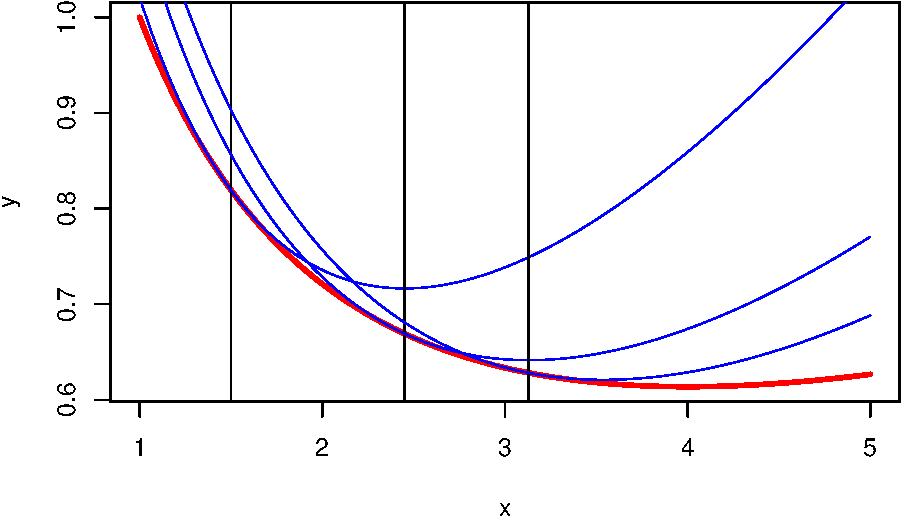
\includegraphics[keepaspectratio]{smacofBA_files/figure-pdf/majplot-1.pdf}}
\end{center}

\subsubsection{Majorizing Stress}\label{majorizing-stress}

\[
\sigma(X)=\frac12\sum w_{ij}(\delta_{ij}-d_{ij}(X))^2=1-\rho(X)+\frac12\eta^2(X)
\]

\begin{lemma}[Cauchy-Schwartz]\protect\hypertarget{lem-cs}{}\label{lem-cs}

For all \(X\) and \(Y\) \[
\rho(X)\geq\text{tr}\ X'B(Y)Y=\text{tr}\ X'V\overline{Y}
\] with equality if \(X=Y\).

\end{lemma}

\begin{proof}
\[
d_{ij}(X)=\sqrt{\text{tr}\ X'A_{ij}X}
\] \[
d_{ij}(X)d_{ij}(Y)\geq\text{tr}\ X'A_{ij}Y
\] If \(d_{ij}(Y)>0\) this \[
d_{ij}(X)\geq\frac{1}{d_{ij}(Y)}\text{tr}\ X'A_{ij}Y
\] If \(d_{ij}(Y)=0\) then \[
d_{ij}(X)\geq b_{ij}\ \text{tr}\ X'A_{ij}Y=0
\]
\end{proof}

\[
\rho(X)=\text{tr}\ X'V\overline X\leq\eta(X)\eta(\overline X)
\] \begin{align}
\sigma(X)&=1+\frac12\eta^2(X-\overline X)-\frac12\eta^2(\overline X),\\
\sigma(X)&\leq 1+\frac12\eta^2(X-\overline X)-\frac12\eta^2(\overline X).
\end{align}

\subsubsection{Accelerating}\label{accelerating}

\[
X^+=\frac12(1+\beta)\overline{X}+\frac12(1-\beta)X
\] Regular smacof \(\beta = 1\). Accelerated \(\beta=3\)

\subsection{Stress formula two}\label{stress-formula-two}

Minorization result

\sectionbreak

\section{smacof Datastructure}\label{smacof-datastructure}

with or without weights

\subsubsection{Metric}\label{metric}

\((i, j, \text{dissimilarity}, \text{weight})\)

\subsection{Interval}\label{interval}

\((i, j, \text{lower bound}, \text{upper bound}, \text{weight})\)

\subsection{Ordinal}\label{ordinal}

\((i, j, \text{tied}, text{weight})\)

\subsection{Paired Comparisons}\label{paired-comparisons}

\((i, j, k, l, \text{tied}, \text{weight})\)

\subsection{Complete triads}\label{complete-triads}

\[(i, j, k, \text{smallest}, \text{largest}, \text{weight})\] \#\#
Indicator

\[(i, l, \text{weight})\]

\sectionbreak

\section{Code}\label{code}

The programs for the techniques discussed in this manual are (currently)
written in R (R Core Team (\citeproc{ref-r_core_team_24}{2024})). There
are plans to translate them, or at least their computational cores, to
C, but I am not sure I'll ever get to that.

The functions in the R files that I wrote are all called smacofFoo,
using Camel Case, where Foo is something more or less descriptive of
what the function is doing. Of course functions that come with R, or
with packages written by others, keep their original names. Plots are
made in ggplot2 ((\citeproc{ref-wickham_}{\textbf{wickham\_?}})), the
manual is written in quarto ().

Each chapter of the manual has one main function implementing the
technique discussed in the chapter. Since the programs share a lot of
code there are many subroutines or modules implementing common
operations. For my private use the code for each chapter is compiled
into a barebones R package.

Almost all programs contain what I call a ``partial iterator''. It is a
piece of code that performs iterations and that looks like

\begin{Shaded}
\begin{Highlighting}[]
\NormalTok{smacofFoo }\OtherTok{\textless{}{-}} \ControlFlowTok{function}\NormalTok{(xold, itmax, eps, verbose, ...) \{}
\NormalTok{  itel }\OtherTok{\textless{}{-}} \DecValTok{1}
\NormalTok{  fold }\OtherTok{\textless{}{-}}\NormalTok{ evaluation xold}
  \ControlFlowTok{repeat}\NormalTok{ \{}
\NormalTok{    xnew }\OtherTok{\textless{}{-}}\NormalTok{ update xold}
\NormalTok{    fnew }\OtherTok{\textless{}{-}}\NormalTok{ evaluation xnew}
    \ControlFlowTok{if}\NormalTok{ (verbose) \{}
      \FunctionTok{cat}\NormalTok{(}
        \StringTok{"itel "}\NormalTok{,}
        \FunctionTok{formatC}\NormalTok{(itel, }\AttributeTok{format =} \StringTok{"d"}\NormalTok{),}
        \StringTok{"fold "}\NormalTok{,}
        \FunctionTok{formatC}\NormalTok{(fold, }\AttributeTok{format =} \StringTok{"f"}\NormalTok{, }\AttributeTok{digits =}\NormalTok{ some number),}
        \StringTok{"fnew "}\NormalTok{,}
        \FunctionTok{formatC}\NormalTok{(fnew, }\AttributeTok{format =} \StringTok{"f"}\NormalTok{, }\AttributeTok{digits =}\NormalTok{ some number),}
        \StringTok{"}\SpecialCharTok{\textbackslash{}n}\StringTok{"}
\NormalTok{      )}
\NormalTok{    \}}
    \ControlFlowTok{if}\NormalTok{ ((}\FunctionTok{test}\NormalTok{(fold, fnew) }\SpecialCharTok{||}\NormalTok{ (itel }\SpecialCharTok{==}\NormalTok{ itmax))) \{}
      \ControlFlowTok{break}
\NormalTok{    \}}
\NormalTok{    itel }\OtherTok{\textless{}{-}}\NormalTok{ itel }\SpecialCharTok{+} \DecValTok{1}
\NormalTok{    xold }\OtherTok{\textless{}{-}}\NormalTok{ xnew}
\NormalTok{    fold }\OtherTok{\textless{}{-}}\NormalTok{ fnew}
\NormalTok{  \}}
  \FunctionTok{return}\NormalTok{(}\FunctionTok{list}\NormalTok{(}\AttributeTok{x =}\NormalTok{ xnew, }\AttributeTok{f =}\NormalTok{ fnew, other results))}
\NormalTok{\}}
\end{Highlighting}
\end{Shaded}

Partial iterators can, and often are, nested, so there are outer, inner,
innermost and so on iterations. Iterators test for convergence, but in
inner iterations they are often called with a small value of itmax, so
they only perform a small number of iterations. They merely improve
their objective, they do not go all the way to the optimum or fixed
point. Many of the iterators depend on alternating least squares (De
Leeuw (\citeproc{ref-deleeuw_C_94c}{1994})). majorization (De Leeuw
(\citeproc{ref-deleeuw_C_94c}{1994})), or MM (Lange
(\citeproc{ref-lange_16}{2016})) to compute these improvements

\sectionbreak

\section*{References}\label{references}
\addcontentsline{toc}{section}{References}

\phantomsection\label{refs}
\begin{CSLReferences}{1}{0}
\bibitem[\citeproctext]{ref-bauschke_bui_wang_18}
Bauschke, H. H., M. N. Bui, and X. Wang. 2018. {``{Projecting onto the
Intersection of a Cone and a Sphere}.''} \emph{SIAM Journal on
Optimization} 28: 2158--88.

\bibitem[\citeproctext]{ref-boehning_lindsay_88}
Böhning, D., and B. G. Lindsay. 1988. {``{Monotonicity of
Quadratic-approximation Algorithms}.''} \emph{Annals of the Institute of
Statistical Mathematics} 40 (4): 641--63.

\bibitem[\citeproctext]{ref-borg_groenen_05}
Borg, I., and P. J. F. Groenen. 2005. \emph{Modern Multidimensional
Scaling}. Second Edition. Springer.

\bibitem[\citeproctext]{ref-deleeuw_R_68d}
De Leeuw, J. 1968. {``Nonmetric Discriminant Analysis.''} Research Note
06-68. Department of Data Theory, University of Leiden.

\bibitem[\citeproctext]{ref-deleeuw_U_75a}
---------. 1975. {``{A Normalized Cone Regression Approach to
Alternating Least Squares Algorithms}.''} Department of Data Theory
FSW/RUL.

\bibitem[\citeproctext]{ref-deleeuw_C_77}
---------. 1977. {``Applications of Convex Analysis to Multidimensional
Scaling.''} In \emph{Recent Developments in Statistics}, edited by J. R.
Barra, F. Brodeau, G. Romier, and B. Van Cutsem, 133--45. Amsterdam, The
Netherlands: North Holland Publishing Company.

\bibitem[\citeproctext]{ref-deleeuw_A_88b}
---------. 1988. {``Convergence of the Majorization Method for
Multidimensional Scaling.''} \emph{Journal of Classification} 5:
163--80.

\bibitem[\citeproctext]{ref-deleeuw_C_94c}
---------. 1994. {``{Block Relaxation Algorithms in Statistics}.''} In
\emph{Information Systems and Data Analysis}, edited by H. H. Bock, W.
Lenski, and M. M. Richter, 308--24. Berlin: Springer Verlag.
\url{https://jansweb.netlify.app/publication/deleeuw-c-94-c/deleeuw-c-94-c.pdf}.

\bibitem[\citeproctext]{ref-deleeuw_E_17e}
---------. 2017. {``{Shepard Non-metric Multidimensional Scaling}.''}
2017.
\url{https://jansweb.netlify.app/publication/deleeuw-e-17-e/deleeuw-e-17-e.pdf}.

\bibitem[\citeproctext]{ref-deleeuw_E_19d}
---------. 2019. {``Normalized Cone Regression.''} 2019.
\url{https://jansweb.netlify.app/publication/deleeuw-e-19-d/deleeuw-e-19-d.pdf}.

\bibitem[\citeproctext]{ref-deleeuw_heiser_C_77}
De Leeuw, J., and W. J. Heiser. 1977. {``Convergence of Correction
Matrix Algorithms for Multidimensional Scaling.''} In \emph{Geometric
Representations of Relational Data}, edited by J. C. Lingoes, 735--53.
Ann Arbor, Michigan: Mathesis Press.

\bibitem[\citeproctext]{ref-deleeuw_heiser_C_80}
---------. 1980. {``Multidimensional Scaling with Restrictions on the
Configuration.''} In \emph{Multivariate Analysis, Volume {V}}, edited by
P. R. Krishnaiah, 501--22. Amsterdam, The Netherlands: North Holland
Publishing Company.

\bibitem[\citeproctext]{ref-deleeuw_heiser_C_82}
---------. 1982. {``Theory of Multidimensional Scaling.''} In
\emph{Handbook of Statistics, Volume {II}}, edited by P. R. Krishnaiah
and L. Kanal. Amsterdam, The Netherlands: North Holland Publishing
Company.

\bibitem[\citeproctext]{ref-deleeuw_mair_A_09c}
De Leeuw, J., and P. Mair. 2009. {``{Multidimensional Scaling Using
Majorization: SMACOF in R}.''} \emph{Journal of Statistical Software} 31
(3): 1--30. \url{https://www.jstatsoft.org/article/view/v031i03}.

\bibitem[\citeproctext]{ref-dempster_laird_rubin_77}
Dempster, A. P., N. M. Laird, and D. B. Rubin. 1977. {``{Maximum
Likelihood for Incomplete Data via the EM Algorithm}.''} \emph{Journal
of the Royal Statistical Society} B39: 1--38.

\bibitem[\citeproctext]{ref-groenen_vandevelden_16}
Groenen, P. J. F., and M. Van de Velden. 2016. {``{Multidimensional
Scaling by Majorization: A Review}.''} \emph{Journal of Statistical
Software} 73 (8): 1--26.
\url{https://www.jstatsoft.org/index.php/jss/article/view/v073i08}.

\bibitem[\citeproctext]{ref-guttman_68}
Guttman, L. 1968. {``{A General Nonmetric Technique for Fitting the
Smallest Coordinate Space for a Configuration of Points}.''}
\emph{Psychometrika} 33: 469--506.

\bibitem[\citeproctext]{ref-kruskal_64a}
Kruskal, J. B. 1964a. {``{Multidimensional Scaling by Optimizing
Goodness of Fit to a Nonmetric Hypothesis}.''} \emph{Psychometrika} 29:
1--27.

\bibitem[\citeproctext]{ref-kruskal_64b}
---------. 1964b. {``{Nonmetric Multidimensional Scaling: a Numerical
Method}.''} \emph{Psychometrika} 29: 115--29.

\bibitem[\citeproctext]{ref-kruskal_carroll_69}
Kruskal, J. B., and J. D. Carroll. 1969. {``{Geometrical Models and
Badness of Fit Functions}.''} In \emph{Multivariate Analysis, Volume
II}, edited by P. R. Krishnaiah, 639--71. North Holland Publishing
Company.

\bibitem[\citeproctext]{ref-lange_16}
Lange, K. 2016. \emph{MM Optimization Algorithms}. SIAM.

\bibitem[\citeproctext]{ref-lethi_tao_18}
Le Thi, H. A., and P. D. Tao. 2018. {``{DC Programming and DCA: Thirty
Years of Developments}.''} \emph{Mathematical Programming, Series B}.

\bibitem[\citeproctext]{ref-mair_groenen_deleeuw_A_22}
Mair, P., P. J. F. Groenen, and J. De Leeuw. 2022. {``{More on
Multidimensional Scaling in R: smacof Version 2}.''} \emph{Journal of
Statistical Software} 102 (10): 1--47.
\url{https://www.jstatsoft.org/article/view/v102i10}.

\bibitem[\citeproctext]{ref-nikolova_ng_05}
Niikolova, M., and M. Ng. 2005. {``Analysis of Half-Quadratic
Minimization Methods for Signal and Image Recovery.''} \emph{SIAM
Journal Scientific Computing} 27 (3): 937--66.

\bibitem[\citeproctext]{ref-r_core_team_24}
R Core Team. 2024. \emph{R: A Language and Environment for Statistical
Computing}. {Vienna, Austria}: R Foundation for Statistical Computing.
\url{https://www.R-project.org/}.

\bibitem[\citeproctext]{ref-shepard_62a}
Shepard, R. N. 1962a. {``{The Analysis of Proximities: Multidimensional
Scaling with an Unknown Distance Function. I}.''} \emph{Psychometrika}
27: 125--40.

\bibitem[\citeproctext]{ref-shepard_62b}
---------. 1962b. {``{The Analysis of Proximities: Multidimensional
Scaling with an Unknown Distance Function. II}.''} \emph{Psychometrika}
27: 219--46.

\bibitem[\citeproctext]{ref-torgerson_52}
Torgerson, W. S. 1952. {``{Multidimensional Scaling: I. Theory and
Method}.''} \emph{Psychometrika} 17 (4): 401--19.

\bibitem[\citeproctext]{ref-vosz_eckhardt_80}
Vosz, H., and U. Eckhardt. 1980. {``{Linear Convergence of Generalized
{W}eiszfeld's Method}.''} \emph{Computing} 25: 243--51.

\bibitem[\citeproctext]{ref-young_81}
Young, F. W. 1981. {``{Quantitative Analysis of Qualitative Data}.''}
\emph{Psychometrika} 46: 357--88.

\bibitem[\citeproctext]{ref-young_deleeuw_takane_C_80}
Young, F. W., J. De Leeuw, and Y. Takane. 1980. {``Quantifying
Qualitative Data.''} In \emph{Similarity and Choice. Papers in Honor of
Clyde Coombs}, edited by E. D. Lantermann and H. Feger. Bern: Hans
Huber.

\bibitem[\citeproctext]{ref-yuille_rangarajan_03}
Yuille, A. L., and A. Rangarajan. 2003. {``{The Concave-Convex
Procedure}.''} \emph{Neural Computation} 15: 915--36.

\bibitem[\citeproctext]{ref-zangwill_69a}
Zangwill, W. I. 1969. \emph{{Nonlinear Programming: a Unified
Approach}}. Englewood-Cliffs, N.J.: Prentice-Hall.

\end{CSLReferences}




\end{document}
